\documentclass[12pt]{article}
\usepackage{times} 			% use Times New Roman font

\usepackage[margin=1in]{geometry}   % sets 1 inch margins on all sides
\usepackage[hidelinks]{hyperref}               % for URL formatting
\usepackage[pdftex]{graphicx}       % So includegraphics will work
\setlength{\parskip}{1em}           % skip 1em between paragraphs
\usepackage{indentfirst}            % indent the first line of each paragraph
\usepackage{datetime}
\usepackage[small, bf]{caption}
\usepackage{listings}               % for code listings
\usepackage{xcolor}                 % for styling code
\usepackage{multirow}

%New colors defined below
\definecolor{backcolour}{RGB}{246, 246, 246}   % 0xF6, 0xF6, 0xF6
\definecolor{codegreen}{RGB}{16, 124, 2}       % 0x10, 0x7C, 0x02
\definecolor{codepurple}{RGB}{170, 0, 217}     % 0xAA, 0x00, 0xD9
\definecolor{codered}{RGB}{154, 0, 18}         % 0x9A, 0x00, 0x12

%Code listing style named "gcolabstyle" - matches Google Colab
\lstdefinestyle{gcolabstyle}{
  basicstyle=\ttfamily\small,
  backgroundcolor=\color{backcolour},   
  commentstyle=\itshape\color{codegreen},
  keywordstyle=\color{codepurple},
  stringstyle=\color{codered},
  numberstyle=\ttfamily\footnotesize\color{darkgray}, 
  breakatwhitespace=false,         
  breaklines=true,                 
  captionpos=b,                    
  keepspaces=true,                 
  numbers=left,                    
  numbersep=5pt,                  
  showspaces=false,                
  showstringspaces=false,
  showtabs=false,                  
  tabsize=2
}

\lstset{style=gcolabstyle}      %set gcolabstyle code listing

% to make long URIs break nicely
\makeatletter
\g@addto@macro{\UrlBreaks}{\UrlOrds}
\makeatother

% for fancy page headings
\usepackage{fancyhdr}
\setlength{\headheight}{13.6pt} % to remove fancyhdr warning
\pagestyle{fancy}
\fancyhf{}
\rhead{\small \thepage}
\lhead{\small HW\#1, Huang}  % EDIT THIS, REPLACE # with HW number
\chead{\small DATA 440, Fall 2022} 

%-------------------------------------------------------------------------
\begin{document}

% EDIT THE ITEMS HERE
\begin{centering}
{\large\textbf{Web Science Intro}}\\ 
Sofia Huang\\
due 09/27/2022\\
\end{centering}

%-------------------------------------------------------------------------

% The * after \section just says to not number the sections
\section*{1.}

\noindent \textbf{Draw the resulting directed graph (either sketch on paper or use another tool) showing how the nodes are connected to each other and include an image in your report. This does not need to fit into the bow-tie type diagram, but should look more similar to the graph on slide 24 from Module-01 Web-Science-Architecture.\\}

\begin{lstlisting}
A --> B
B --> C
C --> D
C --> A
C --> G
E --> F
G --> C
G --> H
I --> H
I --> K
L --> D
M --> A
M --> N
N --> D
O --> A
P --> G 
\end{lstlisting}

\noindent \textbf{For the graph, list the nodes (in alphabetical order) that are each of the following categories:}
\begin{itemize}
\textbf{\item SCC -} A, B, C, G\\
\textbf{\item IN -} M, O, P\\
\textbf{\item OUT -} D, H\\
\textbf{\item Tendrils -} I, K, L (these can reach OUT)\\
\textbf{\item Tubes -} N (connects IN node, M, to OUT node, D)\\
\textbf{\item Disconnected -} E, F\\
\end{itemize}
\clearpage 

Figure \ref{fig:graph} shows the resulting directed graph from the links given.
\begin{figure}[h]
    \centering
    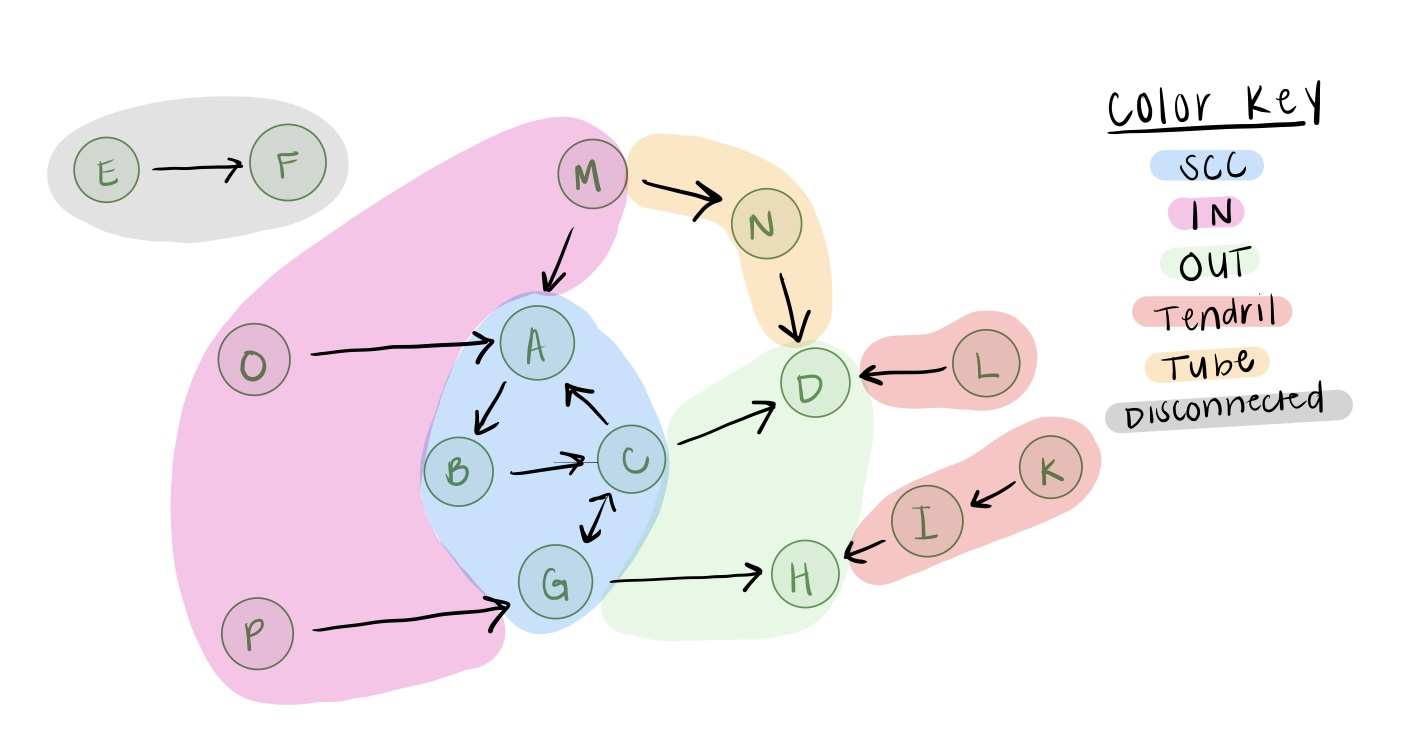
\includegraphics[[width=\textwidth, scale=0.25] {graph.jpg}
    \caption{Bow-tie structure graph}
    \label{fig:graph}
\end{figure}

\noindent To figure out the components of this graph I started with trying to figure out what the SCC was and quickly saw it was comprised of nodes A, B, C, and G. Then, I focused on finding which nodes went into the SCC and had no in-links, those were part of IN. Then, found which nodes came out of the SCC and had no out-links, those were part of OUT. From there, I noticed a node, N, that connected an IN node, M, to an OUT node, D. This is a tube, as it can only be reached from IN, only reach OUT and is not connected to the SCC. Next, I saw that there were some nodes that can only reach OUT nodes: I, L, and K, which means they are tendrils. Lastly, there were two nodes, E and F, that were not connected to any other nodes which made them disconnected.

\section*{2.}
\subsection*{2.1}
\noindent \textbf{First, load this URI https://httpbin.org/user-agent directly in your browser and take a screenshot. The resulting webpage should show the ``User-Agent'' HTTP request header that your web browser sends to the web server.}

Figure \ref{fig:user-agent} shows the resulting web page from the URI: https://httpbin.org/user-agent

\begin{figure}[h]
    \centering
    % trim and clip are used to crop the image, trim=left bottom right top
    % width sets max width, height will be scaled appropriately
    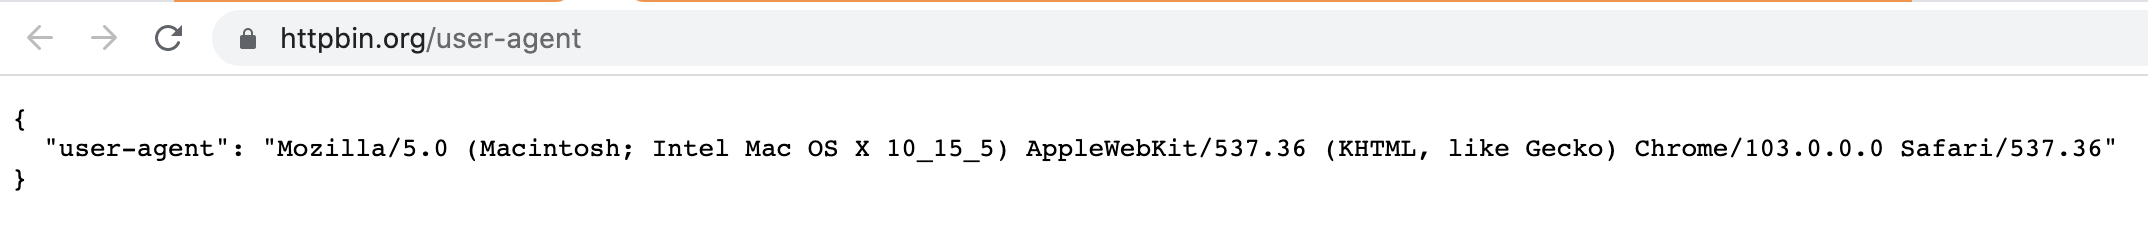
\includegraphics[trim=0 20 10 50, clip, width=\textwidth] {useragent.png}
    \caption{"User-Agent" HTTP request header from my web browser.}
    \label{fig:user-agent}
\end{figure}

According to the Mozilla Developer's definition, a User-Agent is a ``computer program acting as a person''. It identifies the browser, operating system, and version of the browser sending the HTTP request. httpbin.org is an HTTP Request and Response service that allows you to test various HTTP methods, inspect request and response data and much more. So, the specific URI given allows you to see the incoming HTTP request's User-Agent header from my computer. 

\subsection*{2.2}
\noindent \textbf{In a single \lstinline{curl} command, issue a \lstinline{HEAD} HTTP request for the URI, https://t.co/EYgdZgrm2W. Show the HTTP response headers, follow any redirects, and change the User-Agent HTTP request field to ``DATA 440'' Show the command you issued and the result of your execution on the command line. (Either take a screenshot of your terminal or copy/paste into a code segment.)}

\begin{lstlisting}[language=bash, caption=changing User-Agent, label=lst:copy]
(base) sofiahuang@Sofias-MacBook-Pro ~ % curl -A "DATA 440" https://httpbin.org/user-agent

{
  "user-agent": "DATA 440"
}
\end{lstlisting}

To change the user agent, I used the curl argument \lstinline{-A}. Then, using HTTP Bin, the URI given in the previous part, I was able to see that the User-Agent had indeed been changed to what I had set it to, ``DATA 440''. 

\begin{lstlisting}[language=bash, caption=HEAD HTTP request, label=lst:copy]
(base) sofiahuang@Sofias-MacBook-Pro ~ % curl --head -L https://t.co/EYgdZgrm2W
 
HTTP/2 301 
date: Wed, 21 Sep 2022 00:23:29 GMT
vary: Origin
server: tsa_b
expires: Wed, 21 Sep 2022 00:28:29 GMT
location: https://www.nytimes.com/interactive/2022/05/13/us/covid-deaths-us-one-million.html
set-cookie: muc=2600ecf3-30a6-460d-b675-ec7937c4510c; Max-Age=63072000; Expires=Fri, 20 Sep 2024 00:23:29 GMT; Domain=t.co; Secure; SameSite=None
set-cookie: muc_ads=2600ecf3-30a6-460d-b675-ec7937c4510c; Max-Age=63072000; Expires=Fri, 20 Sep 2024 00:23:29 GMT; Path=/; Domain=t.co; Secure; SameSite=None
cache-control: private,max-age=300
strict-transport-security: max-age=0
x-response-time: 7
x-connection-hash: 308b4ffb5d90668ab3f0181710c5c06a9d3b1979cfaa4091d553435a8a40e132

HTTP/2 200 
server: nginx
content-type: text/html; charset=utf-8
x-cloud-trace-context: abacf9e208917890daaf39ca9ef955f1/2148248459137043822
x-b3-traceid: 18ea0a5f3ee84b2dad6725ad1a9de4bd
x-nyt-data-last-modified: Wed, 21 Sep 2022 00:23:29 GMT
last-modified: Wed, 21 Sep 2022 00:23:29 GMT
x-scoop-last-modified: 2022-06-02T20:37:29.713Z
x-pagetype: vi-interactive-minimal
x-xss-protection: 1; mode=block
x-content-type-options: nosniff
cache-control: s-maxage=5,no-cache
x-nyt-route: vi-interactive
x-origin-time: 2022-09-21 00:23:29 UTC
accept-ranges: bytes
date: Wed, 21 Sep 2022 00:23:29 GMT
age: 0
x-served-by: cache-lga21975-LGA, cache-iad-kiad7000045-IAD
x-cache: MISS, MISS
x-cache-hits: 0, 0
x-timer: S1663719809.487903,VS0,VE376
vary: Accept-Encoding, Fastly-SSL
set-cookie: nyt-a=2T5hJtzFuIUuoJMSNjZhi0; Expires=Thu, 21 Sep 2023 00:23:29 GMT; Path=/; Domain=.nytimes.com; SameSite=none; Secure
x-nyt-app-webview: 0
set-cookie: nyt-gdpr=0; Expires=Wed, 21 Sep 2022 06:23:29 GMT; Path=/; Domain=.nytimes.com
x-gdpr: 0
set-cookie: nyt-purr=cfhhcfhhhckfh; Expires=Thu, 21 Sep 2023 00:23:29 GMT; Path=/; Domain=.nytimes.com; SameSite=Lax; Secure
x-frame-options: DENY
onion-location: https://www.nytimesn7cgmftshazwhfgzm37qxb44r64ytbb2dj3x62d2lljsciiyd.onion/interactive/2022/05/13/us/covid-deaths-us-one-million.html
x-api-version: F-F-VI
content-security-policy: upgrade-insecure-requests; default-src data: 'unsafe-inline' 'unsafe-eval' https:; script-src data: 'unsafe-inline' 'unsafe-eval' https: blob:; style-src data: 'unsafe-inline' https:; img-src data: https: blob: android-webview-video-poster:; font-src data: https:; connect-src https: wss: blob:; media-src data: https: blob:; object-src https:; child-src https: data: blob:; form-action https:; report-uri https://csp.nytimes.com/report;
strict-transport-security: max-age=63072000; preload; includeSubdomains
set-cookie: nyt-b3-traceid=18ea0a5f3ee84b2dad6725ad1a9de4bd; Path=/; Domain=.nytimes.com; SameSite=none; Secure
x-nyt-edge-cache: MISS-MISS
content-length: 338478

\end{lstlisting}

When I used the command, \lstinline{curl --head https://t.co/EYgdZgrm2W}, I was able to see that the page had a HTTP response code of 301, meaning the page had been moved permanently. To find the final URI, I used the \lstinline{-L} option to follow the redirects and \lstinline{--head} to show the headers from all requested pages. 

\section*{3.}

\noindent \textbf{Write a Python program to find links to PDFs in a webpage.
Your program must do the following:
\begin{itemize}
\item take the URI of a webpage as a command-line argument
\item extract all the links from the page
\item for each link, request the URI and use the \lstinline{Content-Type} HTTP response header to determine if the link references a PDF file
\item for all links that reference a PDF file, print the original URI (found in the parent HTML page), the final URI (after any redirects), and the number of bytes in the PDF file. (Hint: \lstinline{Content-Length} HTTP response header)
\end{itemize}}


\begin{lstlisting}[language=bash, caption=get\_pdf.py output snippet, label=lst:copy]
(base) sofiahuang@Sofias-MacBook-Pro ~ % python3 /Users/sofiahuang/Desktop/hw1.py http://www.math.wm.edu/~rrkinc/teaching.html
URI: http://www.math.wm.edu/~rrkinc/cs658.pdf
Final URI: http://www.math.wm.edu/~rrkinc/cs658.pdf
Content-Length: 33,524 bytes 

URI: http://www.math.wm.edu/~rrkinc/cs520.pdf
Final URI: http://www.math.wm.edu/~rrkinc/cs520.pdf
Content-Length: 75,028 bytes 

URI: http://www.math.wm.edu/~rrkinc/cs628.pdf
Final URI: http://www.math.wm.edu/~rrkinc/cs628.pdf
Content-Length: 21,434 bytes 

Number of pdf links: 3
\end{lstlisting}

\begin{lstlisting}[language=python, caption=get\_pdf.py code, label=lst:copy]
import requests
from bs4 import BeautifulSoup
import re
import sys
from urllib.parse import urljoin
from urllib3.exceptions import NewConnectionError


def request_url(url):
    # try to request url, catches exception if invalid url is input
    try:
        response = requests.get(url)
    except NewConnectionError:
        print(f'Invalid URL: "{url}"')
    except Exception as e:
        print('There was an exception that occurred when requesting the URL')
        print(e)
        return

    # get html text using BeautifulSoup
    soup = BeautifulSoup(response.text,features="html.parser")
    # counter to track how many pdf links on web page
    pdf_link_count = 0
    # loop through all links on web page
    for links in soup.find_all('a'):
        # make sure the full url is obtained from the href attribute
        href = links.get('href')
        full_url = urljoin(url, href)
        try:
            link_response = requests.get(full_url)
        except Exception as e:
            print('There was an exception that occurred when requesting the URL')
            print(e)
            continue
        # use regex to see if link is a pdf using its content type header
        pattern = re.compile('([a-z]+\/)(pdf)')
        m = pattern.match(link_response.headers['Content-Type'])
        # if link is pdf, print necessary info
        if (m != None):
            # print URI
            print ("URI: {}".format(link_response.url))
            # print final URI, following redirects if necessary
            if (str(link_response.status_code)[0] != '3'):
                print ("Final URI: {}".format(link_response.url))
            else:
                redirect_response = requests.get(link_response.url)
                while (str(link_response.status_code)[0] == '3'):
                    redirect_response = requests.get(link_response.url)
                print ("Final URI: {}".format(redirect_response.url))
            # print content length
            print ("Content-Length: {:,} bytes \n".format(int(link_response.headers['Content-Length'])))
            pdf_link_count += 1
        
    print('Number of pdf links: {}'.format(pdf_link_count))

if __name__ == "__main__":
    # https://alexandernwala.com/files/teaching/fall-2022/week-2/2018_wsdl_publications.html
    # https://haipeng-chen.github.io/
    # http://www.math.wm.edu/~rrkinc/teaching.html
    input_url = str(sys.argv[1])
    request_url(input_url)
\end{lstlisting}

First, I used a try-catch block to request the URL given as input through the command line to make sure the URL is valid. Then, I used BeautifulSoup to get the html and looped through all of the links on the page. For each link, I requested the page, and used regex to see if the link was a pdf by checking the content type. If it was, I printed the URI, followed any redirects, using the status code, to get the final URI, and printed the content length. Finally, I printed the number of pdf links found on the original webpage. I tested the script on Prof. Nwala's publications page, as well as other web pages I found that had pdf links. 

While completing this question, I ran into the problem of not getting the full URL from the \lstinline{href} attribute of the link tag in the html. To fix this, I used \lstinline{urljoin} from the \lstinline{urllib.parse} library so I could request the page.


\section*{References}

\begin{itemize}
    \item {Regex - How to match an optional character} \url{https://stackoverflow.com/questions/4007302/regex-how-to-match-an-optional-character}
    \item {HTTP Bin} \url{https://httpbin.org/user-agent}
    \item {User-Agent} \url{https://developer.mozilla.org/en-US/docs/Glossary/User_agent}
    \item {BS4 - Get full URL in source code}
    \url{https://stackoverflow.com/questions/17972496/using-beautiful-soup-to-get-the-full-url-in-source-code}
    \item {Python Requests - Response Status Codes} \url{https://www.geeksforgeeks.org/response-status_code-python-requests/}
    \item {Q3 - Find PDF links - URI\#1} \url{https://alexandernwala.com/files/teaching/fall-2022/week-2/2018_wsdl_publications.html}
    \item{Q3 - Find PDF links - URI\#2} \url{https://haipeng-chen.github.io/}
    \item{Q3 - Find PDF links - URI\#3} \url{http://www.math.wm.edu/~rrkinc/teaching.html}
\end{itemize}

\end{document}



